%%%%%%%%%%%%%%%%%%%%%%%%%%%%%%%%%%%%%%%%%
% Journal Article
% LaTeX Template
% Version 1.4 (15/5/16)
%
% This template has been downloaded from:
% http://www.LaTeXTemplates.com
%
% Original author:
% Frits Wenneker (http://www.howtotex.com) with extensive modifications by
% Vel (vel@LaTeXTemplates.com)
%
% License:
% CC BY-NC-SA 3.0 (http://creativecommons.org/licenses/by-nc-sa/3.0/)
%
%%%%%%%%%%%%%%%%%%%%%%%%%%%%%%%%%%%%%%%%%

%----------------------------------------------------------------------------------------
%	PACKAGES AND OTHER DOCUMENT CONFIGURATIONS
%----------------------------------------------------------------------------------------

\documentclass[twoside,twocolumn]{article}

\usepackage{blindtext} % Package to generate dummy text throughout this template 

\usepackage[sc]{mathpazo} % Use the Palatino font
\usepackage[T1]{fontenc} % Use 8-bit encoding that has 256 glyphs
\linespread{1.05} % Line spacing - Palatino needs more space between lines
\usepackage{microtype} % Slightly tweak font spacing for aesthetics

\usepackage[english]{babel} % Language hyphenation and typographical rules

\usepackage[hmarginratio=1:1,top=32mm,columnsep=20pt]{geometry} % Document margins
\usepackage[hang, small,labelfont=bf,up,textfont=it,up]{caption} % Custom captions under/above floats in tables or figures
\usepackage{booktabs} % Horizontal rules in tables

\usepackage{lettrine} % The lettrine is the first enlarged letter at the beginning of the text

\usepackage{enumitem} % Customized lists
\setlist[itemize]{noitemsep} % Make itemize lists more compact

\usepackage{abstract} % Allows abstract customization
\renewcommand{\abstractnamefont}{\normalfont\bfseries} % Set the "Abstract" text to bold
\renewcommand{\abstracttextfont}{\normalfont\small\itshape} % Set the abstract itself to small italic text

\usepackage{titlesec} % Allows customization of titles
\renewcommand\thesection{\Roman{section}} % Roman numerals for the sections
\renewcommand\thesubsection{\Roman{section} \Alph{subsection}} % roman numerals for subsections
\titleformat{\section}[block]{\large\scshape\centering}{\thesection.}{1em}{} % Change the look of the section titles
\titleformat{\subsection}[block]{\large}{\thesubsection.}{1em}{} % Change the look of the section titles

\usepackage{fancyhdr} % Headers and footers
\pagestyle{fancy} % All pages have headers and footers
\fancyhead{} % Blank out the default header
\fancyfoot{} % Blank out the default footer
\fancyhead[C]{State of Art of Artificial Neurals Networks Compression} % Custom header text
\fancyfoot[RO,LE]{\thepage} % Custom footer text

\usepackage{titling} % Customizing the title section

\usepackage{hyperref} % For hyperlinks in the PDF

\usepackage{amsmath,array}
\newcommand*{\vertbar}{\rule[-1ex]{0.5pt}{2.5ex}}
\newcommand*{\horzbar}{\rule[.5ex]{2.5ex}{0.5pt}}

\usepackage{graphicx}
\graphicspath{ {./images/} }
%----------------------------------------------------------------------------------------
%	TITLE SECTION
%----------------------------------------------------------------------------------------

\setlength{\droptitle}{-4\baselineskip} % Move the title up

\pretitle{\begin{center}\Huge\bfseries} % Article title formatting
\posttitle{\end{center}} % Article title closing formatting
\title{State of Art in Artificial Neurals Networks Compression} % Article title
\author{%
\textsc{Pierre Gabin FODOP GUMETE} \\[1ex] % Your name
\normalsize ENSTA Bretagne \\ % Your institution
\normalsize \href{mailto:pierre.fodop@ensta-bretagne.org}{pierre.fodop@ensta-bretagne.org} % Your email address
%\and % Uncomment if 2 authors are required, duplicate these 4 lines if more
%\textsc{Jane Smith}\thanks{Corresponding author} \\[1ex] % Second author's name
%\normalsize University of Utah \\ % Second author's institution
%\normalsize \href{mailto:jane@smith.com}{jane@smith.com} % Second author's email address
}
\date{\today} % Leave empty to omit a date
\renewcommand{\maketitlehookd}{%
\begin{abstract}
  In the last twenty years, we have seen an exponential increase in the computing power of personal computers, in addition 
  to the explosion of cloud services and the increase in the number of server farms for data storage. One of the 
  consequences of this increase was to make a certain amount of data available to as many people as possible, but also 
  the explosion of Neural Networking methods with the objective of use this data. They have been applied to a large 
  number of problems, in particular in image processing, sound processing, natural language processing (...) Areas in 
  which they currently constitute the state of the art. On the other hand, we have also had a significant advance in the 
  Internet of Things, which creates the need for neural networks adapted to powerful objects. The objective of this article 
  is to present the different methods to compress neural networks and thus store networks in a smaller space, but also to 
  accelerate calculations with them.
\end{abstract}
}

%----------------------------------------------------------------------------------------

\begin{document}

% Print the title
\maketitle

%----------------------------------------------------------------------------------------
%	ARTICLE CONTENTS
%----------------------------------------------------------------------------------------

\section{Introduction}
The history of neural networks begins with Warren S. McCulloch and Walter Pitts of MIT researchers who presented in 1943 an
article on the realization of neural functions by electrical functions and logic gates.\cite{warren1}.
Their approach is linked to a perception of neuronal functions as {\bf\textit{all or nothing}} functions. 
This advance will be completed later by the definition of the perceptron\cite{RosenBlatt1} and the discovery of the gradient 
back-propagation algorithm\cite{Rumelhart1}.

\begin{figure}[h]
\centering
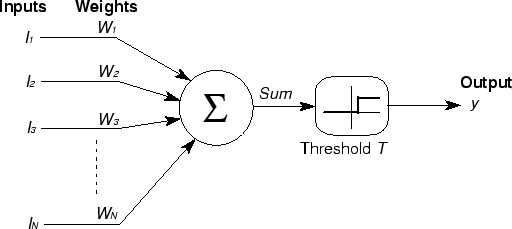
\includegraphics[width=70mm]{CulochNeurone.png}
\caption{McCulloch and Pitts Computational Model}
\label{SimpleNeuron}
\end{figure}

With the \textit{winter of arrtificial l'Intelligence} which will begin at the end of the 1960s, advances in the field of 
artificial intelligence will be slower.Also because of a reduction in both public and private investments in this field. 
Although slowed down, it was during this period that the first large-scale implementations of expert systems designed in 
1950 were designed. Here, most intelligent systems work with a so-called \textit{Knowlege Based} base. We have the development 
of the bases of methods such as Inductive Logic Programming (ILP)\cite{Muggleton1}\cite{Ehud1}. Which will later be compiled 
by S.H. Muggleton in his founding article "Inductive Logic Programming"\cite{Muggleton2}.

Finally, in the 1990s, there was a comeback of artificial intelligence with new methods and with the increase in computing power; 
this with the advent of the first Pentium processors by Intel, a generalization of supercomputers and finally the advent of the 
Internet which will allow an unprecedented exchange of knowledge. This evolution will reach a first major palliative in 2012 with 
the application of neural networks to the ImageNet image classification challenge which will make it possible to reduce the lowest 
rate of classification error from 25 \% to 16 \% thanks to the AlexNet network\cite{Rajat1}. 

Since then, neural networks have been applied to an increasing number of problems. especially in Computer Vision\cite{MadhusmitaSahu}
\cite{Sornaminproceedings}, en Natural language processing\cite{jing2019survey}, in signal analysis\cite{MohamedIbn1}\cite{XiaofanLi1} 
an other. \cite{POZNYAK2019250} With better results than the methods that were used until then. This has created the need for neural 
networks suitable for a certain number of supports. In particular media from the Internet of Things.

The objective of this document is to make a tour of the methods allowing to compress neural networks and to apply them in a certain number 
of objects, to do this, we will start by making a presentation of the different existing neural network architectures. , then, we will 
explore the methods of pruning, sparse representation in particular quantified, knowledge distillation and finally, we will see the future methods

%------------------------------------------------

\section{Types of Neurals Networks}

\subsection{The Perceptron}

It is the simplest expression of a neural network, it consists of a single formal neuron\cite{warren1}.

\begin{figure}[h]
  \centering
  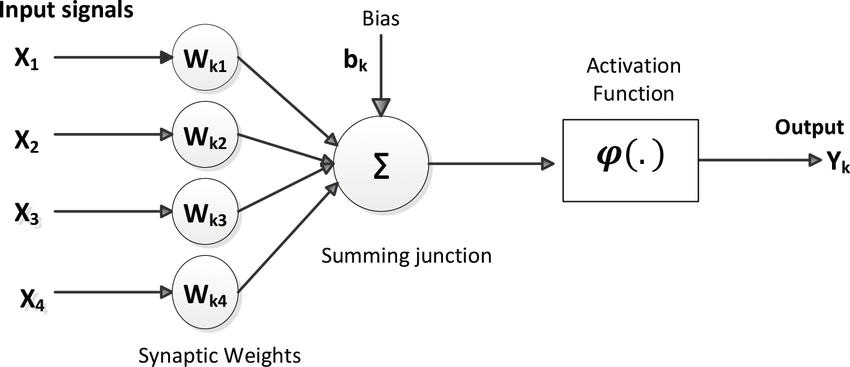
\includegraphics[width=70mm]{McCulloch-Pitts-computational-model-of-a-neuron.png}
  \caption{Simple Perceptron }
  \label{PerceptronMathematique}
\end{figure}

The neuron took as input a vector of values $x$, multiply then with a weigth vector $w$ finally thanks to the activation function returns 
the exit to us.
\[
y = \varphi(
\left[
  \begin{array}{ccc}
    w_{1}\\
    w_{2}\\
    w_{3}\\
    w_{4}\\  
  \end{array}
\right]*
\begin{bmatrix}
           x_{1} \\
           x_{2} \\
           x_{3} \\
           x_{4}
         \end{bmatrix}
+ b)\]
The activation function $\varphi()$ must meet a number of conditions.
\begin{itemize}
  \item \textbf{Identity in zero} si $f(x) = 0$ alors $x = 0$ \cite{Sussillo2014RandomWI} These functions allow you to make learning more 
  quickly.
  \item \textbf{Monotonic value derivative}\cite{WU20093432} for a better generalization capacity and an ease of application of the convex 
  optimization methods.
  \item \textbf{Everywhere Differentiable}\cite{Rumelhart1} allowing the application of gradient descent.
\end{itemize}

To update the weights $ w $ of our perceptron, we will use the gradient descent algorithm. The latter allows, from a chosen error function, 
to update these weights.Let $ F (x) $ be a defined and differentiable function close to the local minimum point $ a $. The objective is to 
estimate the value of a; we will define a learning coefficient $ \ lambda $. We will therefore define the following sequence with an 
initialization at $ a_0 $.

\[\left\{
  \begin{array}{rcr}
    a_{0} & =  a_0 \\
    a_{n+1} & = & a_{n} - \lambda. \Delta F(a_n)\\
  \end{array}
\right.\]

For a neuron network with the sigmoid function as an activation function and the \textit{cross entropy loss} function as an loss function.

$E(y) = -(y^v.log(y) + (1-y^v).log(1-y))$
\[ \frac{\partial E}{\partial w}
   = \frac{\partial E}{\partial y}
   *\frac{\partial y}{\partial z}
      *\frac{\partial z}{\partial w}\]

\[ \frac{\partial E}{\partial y}
  =  \frac{y^v}{y} - \frac{1-y^v}{1-y}
  = \frac{y^v - y}{y(1 - y)} \]

\[ \frac{\partial y}{\partial z}
  =  y*(1-y) \]

\[ \frac{\partial z}{\partial w}
  =  w^T \]

\[ \frac{\partial E}{\partial w}
  = x*(y^v-y) \]

Where we had 
\[\left\{
  \begin{array}{rcr}
    w_{0} & =  w_0 \\
    w_{n+1} & = & w_{n} - \lambda.(y^v-y).x\\
  \end{array}
\right.\]
The procedure is identical for updating the biases.

At its exit, a neuron makes it possible to classify a class into two classes of values. Those which activate the neurons and those which do 
not activate it; more than one can be used to classify into a larger number of classes. We will then obtain multi-layer perceptrons

\subsection{The Multi-Layer perceptrons}
This is the most basic type of neural network, it is made up of a certain number of layers itself made up of formal neurons.\cite{warren1}. 
The information is thus transmitted from the first layer called the input layer to the last layer called the output, passing through the cache 
layers through the connection between the neurons. In the case where each neuron of a layer is linked to all the neurons of the following 
layer, we speak of fully connected networks.

\begin{figure}[h]
  \centering
  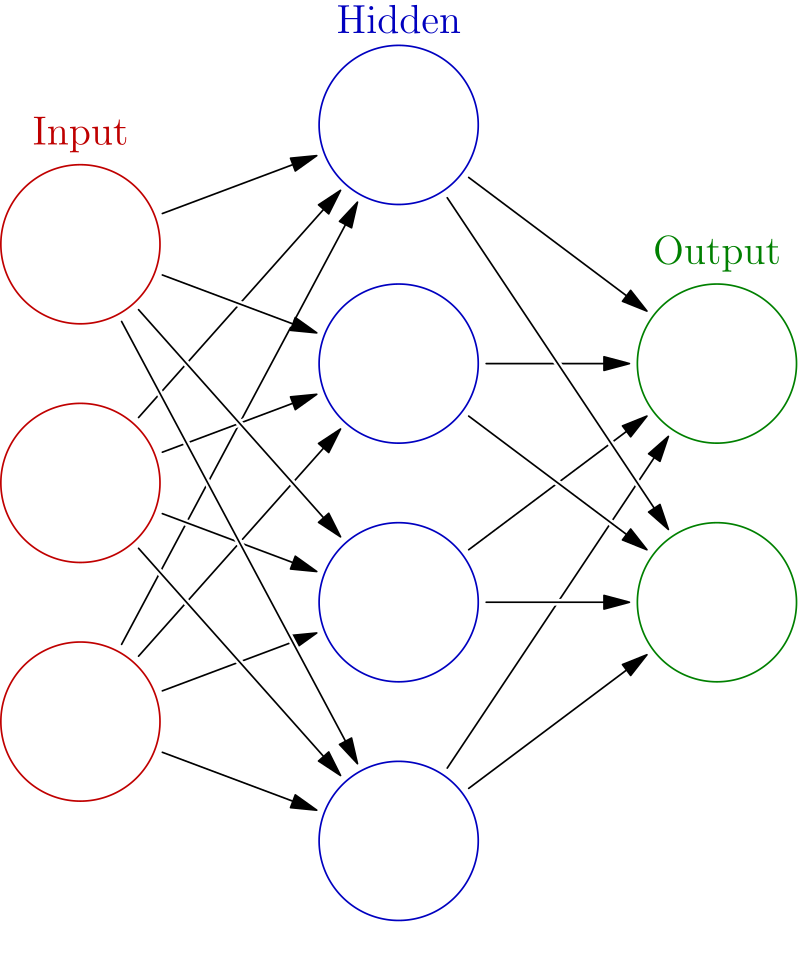
\includegraphics[width=60mm]{Colored_neural_network.png}
  \caption{Multi-Layer perceptrons}
  \label{PerceptronMulticouche}
  \end{figure}
Currently, multi-layered perceptrons, under the best conditions, obtain an error rate of less than 0.35 \%\cite{DeepBig} The mathematical equivalent 
of a network with 784 input 16 caches and 10 output neurons is as follows:

\[
y^1 = \varphi_1(
\left[
  \begin{array}{ccc}
    w_{1}^{1} & ... & w_{1}^{784}\\
    \vdots & \vdots & \vdots\\
    w_{16}^{1} & ... & w_{16}^{784}\\
  \end{array}
\right]*
\begin{bmatrix}
           x_{1} \\
           \vdots \\
           x_{784}
         \end{bmatrix}
+ \begin{bmatrix}
  b_{1} \\
  \vdots \\
  b_{784}
\end{bmatrix}
)\]

\[
y^2 = \varphi_2(
\left[
  \begin{array}{ccc}
    w_{1}^{1} & ... & w_{1}^{16}\\
    \vdots & \vdots & \vdots\\
    w_{10}^{1} & ... & w_{10}^{16}\\  
  \end{array}
\right]*
\begin{bmatrix}
           x_{1} \\
           \vdots \\
           x_{10}
         \end{bmatrix}
+ \begin{bmatrix}
  b_{1} \\
  \vdots \\
  b_{10}
\end{bmatrix}
)\]
To make a probabilistic distribution of the outputs, we can use a certain number of functions, in this case we will use a softmax function.

\[
out = softmax(y^2)
\]
we will therefore have a vector of 10 probabilities, which each signifies if the class represented is the adequate class.


\subsection{Convolutionnals Neurals Networks (CNNs)}
%------------------------------------------------
The greatest flaw of multi-layered perceptron-type networks is their inability to process an image as aggregate information has led to the 
development of Convolutional neural networks.

Filtering for an image is a mathematical operation that allows a matrix called a kernel to do a number of operations on an image. One can 
quote among these last the blurring, the detection of contour. This will be done by convolution of a matrix called nucleus with an our image. 
its mathematical representation is as follows:

\[g(x,y) = w*f(x,y)\]
\[w*f(x,y) = \sum_{dx=-a}^{a} \sum_{dx=-b}^{b} w(dx,dy)f(x+dx,y+dy)\]

In the context of contour detection which is one of the bases of convolutional neural networks, Canny filtering will preferably be used\cite{Canny1}.

\begin{figure}[h]
  \centering
  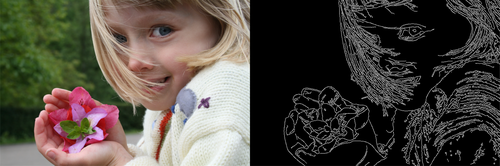
\includegraphics[width=60mm]{canny.png}
  \caption{Canny Filtering}
  \label{CannyOutput}
  \end{figure}

For a convolutional layer, we will apply to our image a certain number of convolutional filters which will allow us to capture as much information 
as possible on the image. We will be able to apply a Pooling on the filtered images obtained to reduce the number of dimensions.

  \begin{figure}[h]
  \centering
  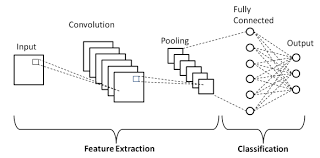
\includegraphics[width=72mm]{convneural.png}
  \caption{Convolutionnal Network}
  \label{ConvNet}
\end{figure}
And at the end of the network, we apply a Multi layer perceptrons network to classify the images. It is also possible to have a fully convolutional network. 

There are many applications of convolutional networks, as much in image processing \cite{Browne1} (VGG16, LeNet, ...), as in natural language processing 
\cite{8666928}, or in audio signal processing \cite{Gama_2019}. Although convolutional neural networks complement perceptron networks, they have the limitation 
of not taking into account temporal values and are quite useful for analyzing sequences such as video sequences.


\subsection{Recurents Neurals Networks}

Les reseaux recurents, on ete cree pour permettre un transfert de l'information dans les cellules en prenant en compte l'infulence du temps. 
Ici on parle d'une double propagation spaciaux temporelle. Cela donne la capacite a ces neuronnes d'intervenir dans l'analyse des phenomene evoluant dans le temps comme les videos, les series temporelles ...

Les reseaux recurents on vu le jour avec le reseau de Hopfield\cite{Hopfield}. Ce dernier introduit la memoire dans les reseau permetant un passage au traver le temps des informations.Ils connaitrons quelques evolutions jusqu'a l'arive d'un autre type 
de reseaux de neurone, Le \textit{Long Short Term Memory}\cite{lstm1}

\begin{figure}[h]
  \centering
  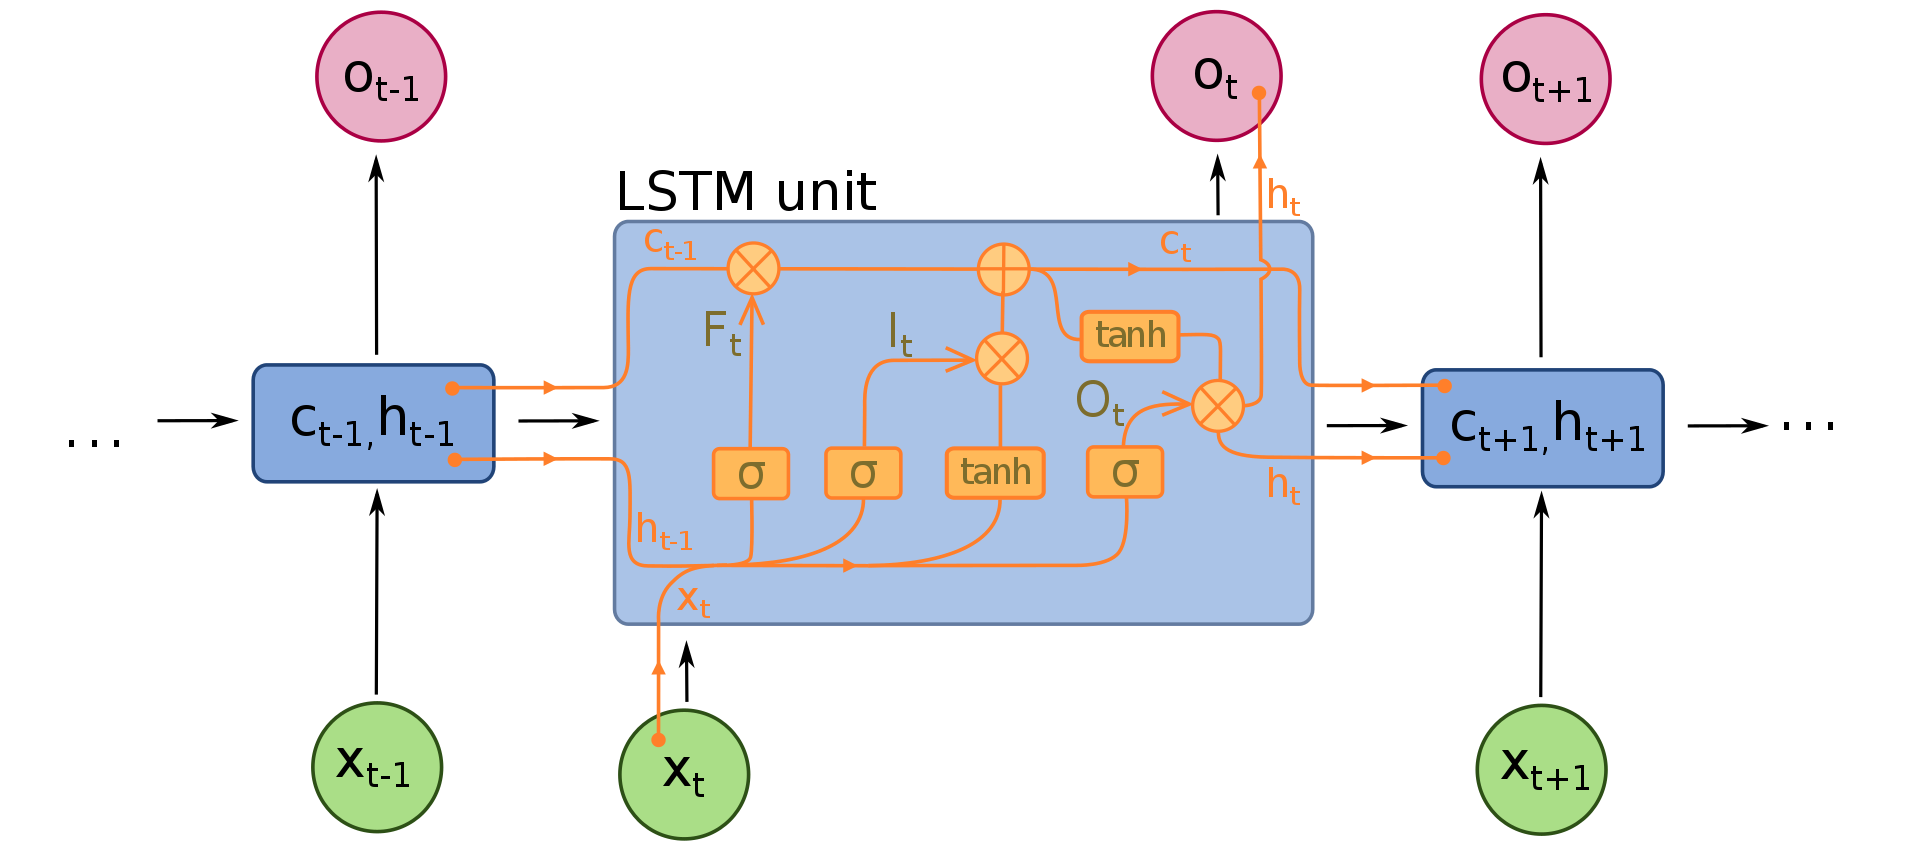
\includegraphics[width=72mm]{Long_Short-Term_Memory.png}
  \caption{Cellule LSTM}
  \label{lstm}
\end{figure}

Une celule LSTM prend en entree 3 valeurs valeurs, les sorties de la celule precedente $H_t$ l'etat cache et $C_t$ l'etat de la celule; mais aussi la valeur actuelle d'entree $X_t$. 

la premiere porte que nous verons est porte de l'oublie. la fonction de la porte d'oublie est la suivante:
\[f_t = \sigma(U^fX_t + W^fh_{t-1})\]
Les portes suivantes permettent de calculer l'etat d'entree et l'etat de sortie
\[i_t = \sigma(UX_t + Wh_{t-1})\]
\[O_t = \sigma(U^{\circ}X_t + W^{\circ}h_{t-1})\]
La porte de sortie
\[g_t = tanh(U^gX_t + W^gh_{t-1})\]
etat final de la cellule
\[c_t = i_tg_t + f_tc_{t-1}\]
Et l'etat cache suivant
\[h_t = tanh(c_t)o_t\]

Enfin en 2014 seront introduit les celule dites Gated Recurrent Unit (GRUs)\cite{cho2014learning}. 

\begin{figure}[h]
  \centering
  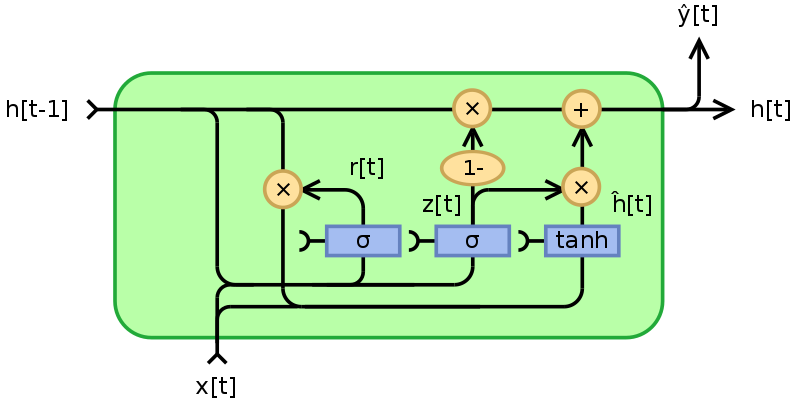
\includegraphics[width=70mm]{GRU.png}
  \caption{Cellule GRU}
  \label{GRUs}
\end{figure}

La cellule GRU prend en entre 2 variables et genere deux sorties. Les entrees sont $h_t$ l'etat cache provenant de la precedente cellule 
$x_t$ la valeur actuelle de l'entree ; les sorties sont quant a elles, $y^est$ la valeur de sortie estimee et $h_t$ l'etat cache estime.

Du point de vue mathematique on a:
\[z_t = \sigma_g(W_{z}x_{t} + U_{z}h_{t-1} + b_{z})\]
\[r_t = \sigma_g(W_{r}x_{t} + U_{r}h_{t-1} + b_{r})\]
\[h_{t}^{est} = \phi_h(W_{h}x_{t} + U_{h}(r_t * h_{t-1}) + b_{h})\]
\[h_t = (1 - z_t)*h_{t-1} + z_t*h_{t}^{est}\]
ou $x_t$ est le vecteur d'entree, $h_t$ le vecteur de sortie, $z_t$ le vecteur de mise a jour des protes, $r_t$ vecteur de reinitialisation, $h_t^{est}$ Vecteur candidat d'acivaion.
$W$, $U$ et $b$ sont les marices de parametre. $\sigma_g$ est la fonction sigmoide et $\phi_h$ est la tangente hyperbolique.

Plus recement, les GRU ont ete modifie pour donner les reseaux Minimal Gated Unit \cite{heck2017simplified}\cite{zhou2016minimal}. Ces reseaux presentent l'avantage d'avoir un minimum
d'entree de sortie et de porte logiques.

\begin{figure}[h]
  \centering
  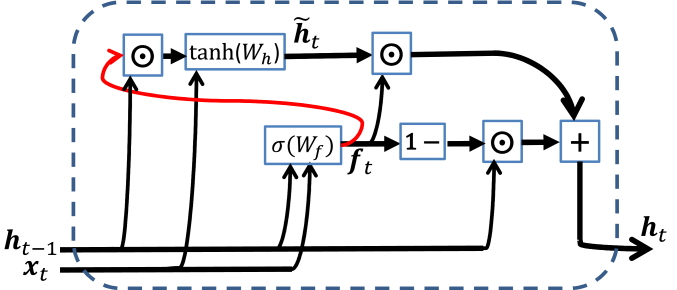
\includegraphics[width=70mm]{MRU.png}
  \caption{Cellule MRU}
  \label{MRUs}
\end{figure}

\subsection{Autres reseaux}
Les types de reseaux de neurones presente plus haut on tous la particularite d'etre en apprendtissage supervise. Ce genre  de reseaux est generalement utilise pour la classification.
Dans cette partie nous nous interesserons au cas des autres types de reseaux dont l'apprentissage est generalement non supervisee. 

les premiers de ces reseaux seront, \textbf{Les Machines de Bolztmann}. l'origine de ces reseaux est l'article de Hinton et Sejnowski de 1983\cite{Rumelhart2}, ils sont utilise pour avoir des estimation de distribution
probabiliste d'un jeux de donnee\cite{Salakhutdinov}. Ces derniers sont generalement utilise sous la forme de machine de bolzmann restreinte a deux couches de neurones. 

En suite nous avons les \textbf{chaines de Markov}, Il s'ait ici d'un reseaux qui a base de connaisance de l'etat actuelle et d'un ensemble de probabilite connue peut predire les etat futur. Elles sont utilise sur les 
processus a temps discret, ou a temps continu et a espace d'etats discret.

Enfin nous classeron un certain nombre de reseaux notemment les auto encodeur (auto-encodeur variationnel, auto encodeur de debruitage), les Reseaux generatifs adversariaux (...) dans la cathegorie des reseaux composees
en cela qu'il sont issue de la composition d'un certain nombre de couche de neuronne issue des reseaux mentionne plus haut.

\section{Pourquoi la compression des reseaux de neurones}%----------
L'origine des objets connectes remonte a 1994 quand la start-up Violet a lance le concept de la lampe connecte en wifi DAL. Et depuis lors leur nombre n'a pa arrete de croitre, leur usage aussi. D'un autre cote le nombre d'outils 
informatique a lui aussi augmente de facons considerable, avec l'invention des smartphones, des tabletes et autres.

Ces objets connnectes ont pour point commun de ne disposer ni d'une grande puissance de calcul ni d'un grand espace de stockage. Cette situation les eloignes des possiblite d'aplication des reseaux de neurones qui quand a eu on besoin
d'une puissance de calcule importante et d'un espace de stockage lui aussi grand.

\begin{table}[!h]  
\begin{tabular}{|l|c|r|}
    \hline
    DNN & Size(MB) & Temps(Milion) \\
    \hline
    AlexNet & 200 & 720 \\
    VGG-16 & 550 & 15 300 \\
    GoogLeNet & 50 & 1550 \\
  ResNet & 170 & 11 300 \\
  \hline
\end{tabular}
\caption{Les Poids et temps de calcul de differents reseaux}
\end{table}

Pour rendre ces objet plus intelligent il est donc important pour nous de pouvoir developper des reseaux de neurones adaptés. Pour ce faire, 
un certain nombre de moyens et de methodes ont ete developpe. Parmi les methodes qui s'attaquent a reduire le poid des reseaux on a, Le pruning, la quantification, la distillation de connaisance.
D'autres approches visent une repartition des calclus entre plusieurs objets comme l'apprentissage federe. Nous explorerons ici en profondeur les approches qui 
s'attellent a reduire la taille des reseaux et nous ferons une introduction de l'aprentissage federe. Enfin , Dans la mesure ndu possible, nous presenterons les resultas que nous avons eu en 
modelisant les methodes.

\section{Le Pruning} %-------------------------------

\subsection{C'est quoi le Pruning}
L'une des premieres idee pour reduire la taille des reseaux en memoire, est de suprimer les connections inutiles entre les neurones.
En effet lors de l'entrainement des reseaux de neurones et leur utilisation, ils existent potentiellement des connections qui se sont jamais 
activee, leurs supression  fait donc gagner de l'espace de stockage.

Le Pruning est la methode de reduction de taille des reseaux de neurones qui consiste a suprimer les poids inferieure a un certain seuil.

\begin{figure}[h]
  \centering
  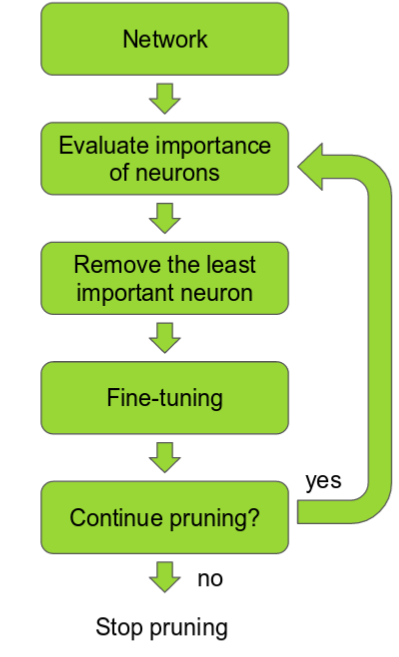
\includegraphics[width=40mm]{pruning_steps.png}
  \caption{etapes de Pruning}
  \label{Pruning_step}
\end{figure}

\begin{figure}[h]
  \centering
  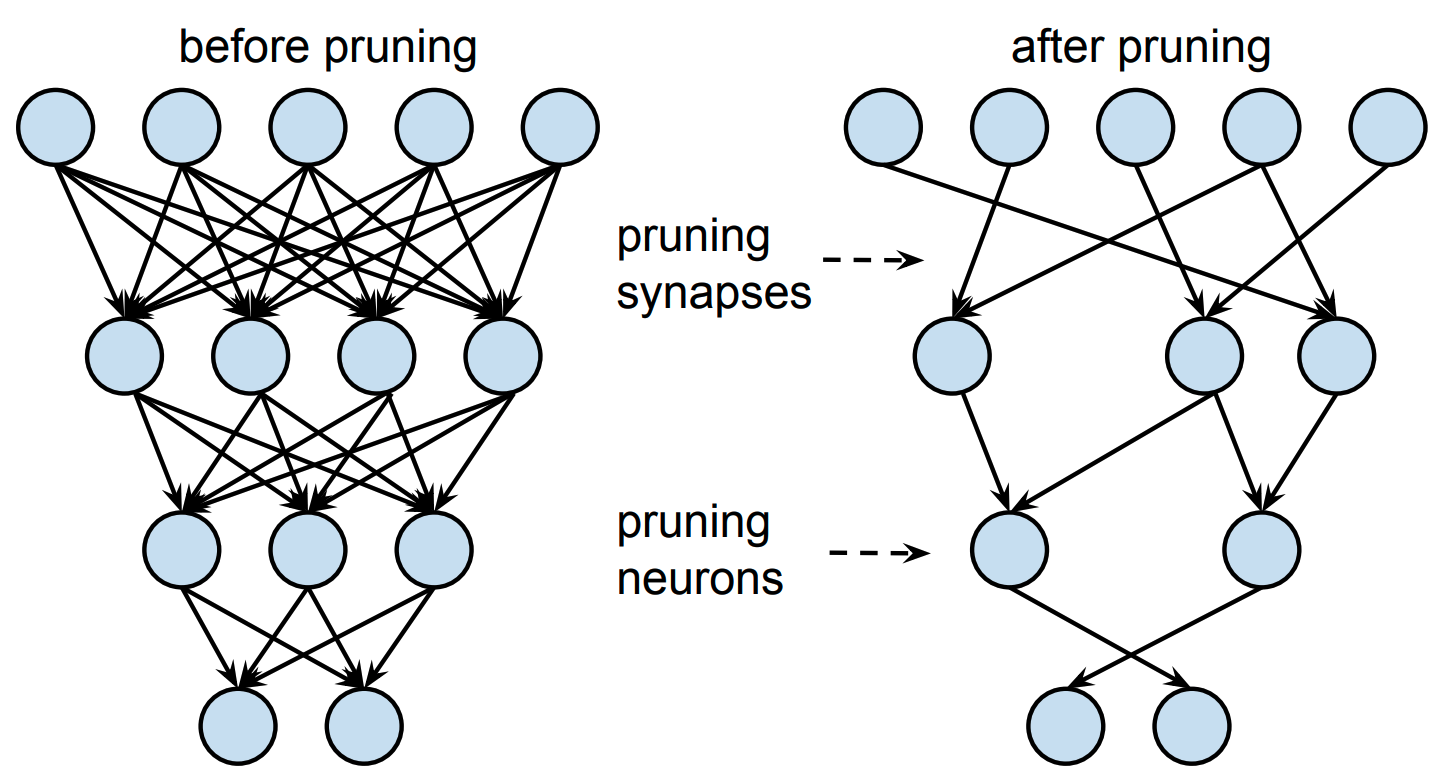
\includegraphics[width=70mm]{pruning.png}
  \caption{Pruning}
  \label{pruning du perceptron Multicouche}
\end{figure}
Les recherches dans ce dommaine sont oriente vers la resolution du probleme compression/ efficacite qui en decoule. 

Dans la section qui suit, nous presenterons l'etat de l'art de la methode de pruning cela en nous  attardant sur certaines publications
que nous avons selectionnee.

\subsection{Etat de l'art de la methode Pruning}
La premiere publication majeure qui a pose les jalon de l'application de la methode de pruning nous date des annee 1991\cite{SYKung}. l'idee principale de ce dernier est 
d'utiliser le mean square error associer a la norme de Forbenius pour 

\subsection{Le futur du Pruning}
\subsection{Presentation de mes resultats}

\section{Quantification}%---------------------
\subsection{Quantification}
\subsection{Binarization}

\section{Distillation de connaissance} %--------------


\section{Autres Methodes}%-----------


\section{Conclusion}%---------

%----------------------------------------------------------------------------------------
%	REFERENCE LIST
%----------------------------------------------------------------------------------------

\bibliographystyle{plain}
\bibliography{reference} 

%----------------------------------------------------------------------------------------

\end{document}
